% !TeX root = ../main.tex
% Add the above to each chapter to make compiling the PDF easier in some editors.

\chapter{Theoretical Foundations}\label{chapter:theoretical_foundations}

This chapter provides the theoretical background necessary to understand the clinical and technical aspects of stroke imaging and analysis.

\section{Ischemic Stroke Pathophysiology}

In ischemic stroke, a blood clot obstructs blood flow to a region of the brain, leading to oxygen and nutrient deprivation in the affected area. The brain tissue affected by a stroke can be categorized into two main regions:

\begin{itemize}
    \item \textbf{Infarct Core}: The central region of severely reduced blood flow where brain cells have already died or are irreversibly damaged.
    
    \item \textbf{Penumbra}: The surrounding area of compromised but still viable brain tissue, which can potentially be saved with timely intervention.
\end{itemize}

The concept "Time is Brain" emphasizes that as time progresses, the infarct core expands at the expense of the penumbra, making rapid diagnosis and treatment essential to preserve brain function.

\section{Imaging Modalities in Stroke}

\subsection{Computed Tomography (CT)}

CT imaging is the first-line imaging modality in acute stroke care due to several advantages:

\begin{itemize}
    \item Faster acquisition (minutes vs. 30-45 minutes for MRI)
    \item Widespread availability in hospitals
    \item No contraindications related to metal implants or pacemakers
    \item No requirement for patients to remain completely still
    \item Cost-effectiveness
    \item Ability to quickly differentiate between ischemic and hemorrhagic stroke
\end{itemize}

However, CT provides primarily structural and anatomical information and is less sensitive than MRI for detecting early ischemic changes.

\subsection{Magnetic Resonance Imaging (MRI)}

MRI is commonly used for follow-up imaging due to:

\begin{itemize}
    \item Superior soft tissue contrast
    \item More accurate visualization of the final infarct volume
    \item Ability to detect even small ischemic lesions
\end{itemize}

Diffusion-weighted imaging (DWI) is particularly valuable, as it is the only imaging technique that reliably demonstrates parenchymal injury within minutes to hours from stroke onset.

\section{Perfusion CT Analysis}

\subsection{Perfusion Maps}

Perfusion maps and imaging techniques:
\begin{itemize}
  \item Derived volumetric data visualizing blood perfusion parameters, not raw CT.
  \item CBF (Cerebral Blood Flow): Blood flow per time through a brain volume (ml/100g tissue/min).
  \item CBV (Cerebral Blood Volume): Total blood volume in a brain region (ml/100g tissue).
  \item MTT (Mean Transit Time): Average time for blood to pass through a region.
  \item TTP (Time to Peak): Time to maximum contrast agent concentration in an area.
  \item Tmax (Time to Maximum): Delay until peak of tissue residue function, sensitive indicator for hypoperfusion.
  \item CTA (Computed Tomography Angiography): CT imaging with contrast agents to visualize vascular structures and detect pathologies.
  \item CTP (Computed Tomography Perfusion): Dynamic CT method quantifying brain perfusion through temporal contrast distribution analysis.
\end{itemize}

\begin{figure}[htbp]
    \centering
    \begin{subfigure}[t]{0.3\textwidth}
        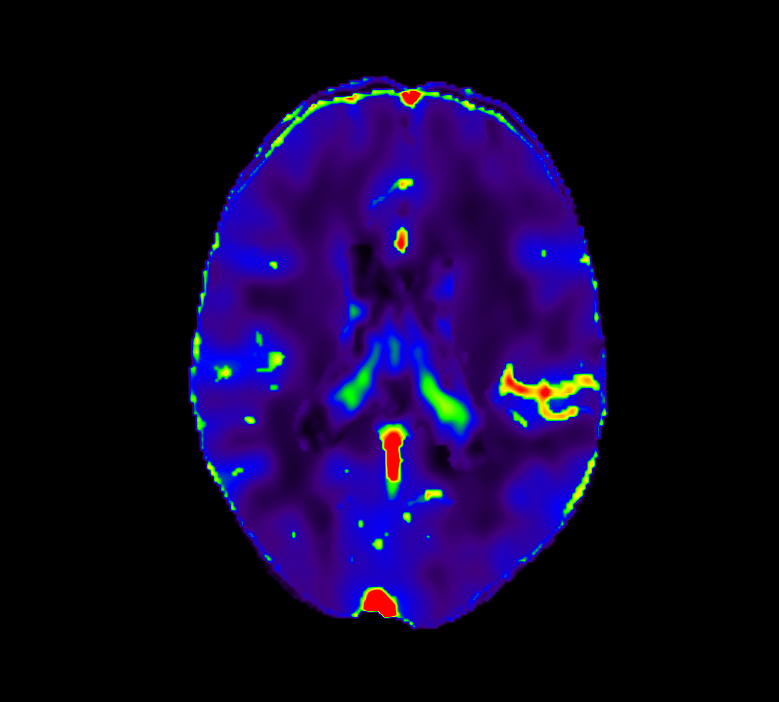
\includegraphics[width=\textwidth,height=4cm,keepaspectratio]{figures/perfusion_cbf.png}
        \caption{Cerebral Blood Flow (CBF) map}
        \label{fig:cbf}
    \end{subfigure}
    \hfill
    \begin{subfigure}[t]{0.3\textwidth}
        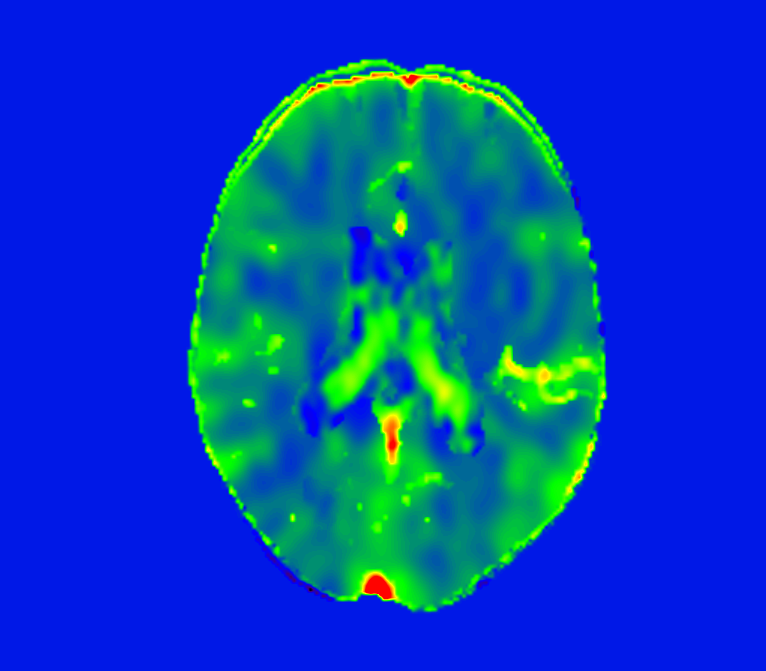
\includegraphics[width=\textwidth,height=4cm,keepaspectratio]{figures/perfusion_cbv.png}
        \caption{Cerebral Blood Volume (CBV) map}
        \label{fig:cbv}
    \end{subfigure}
    \hfill
    \begin{subfigure}[t]{0.3\textwidth}
        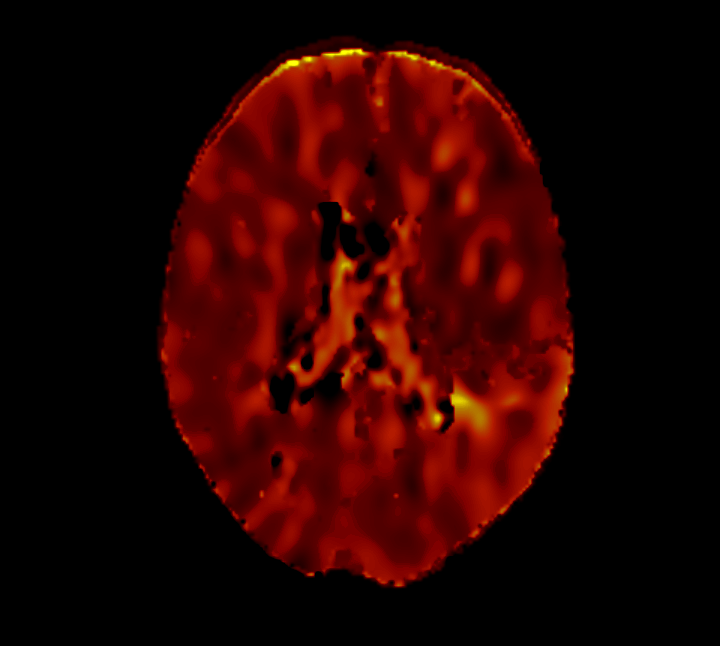
\includegraphics[width=\textwidth,height=4cm,keepaspectratio]{figures/perfusion_mtt.png}
        \caption{Mean Transit Time (MTT) map}
        \label{fig:mtt}
    \end{subfigure}
    
    \vspace{0.5cm}
    
    \begin{subfigure}[t]{0.3\textwidth}
        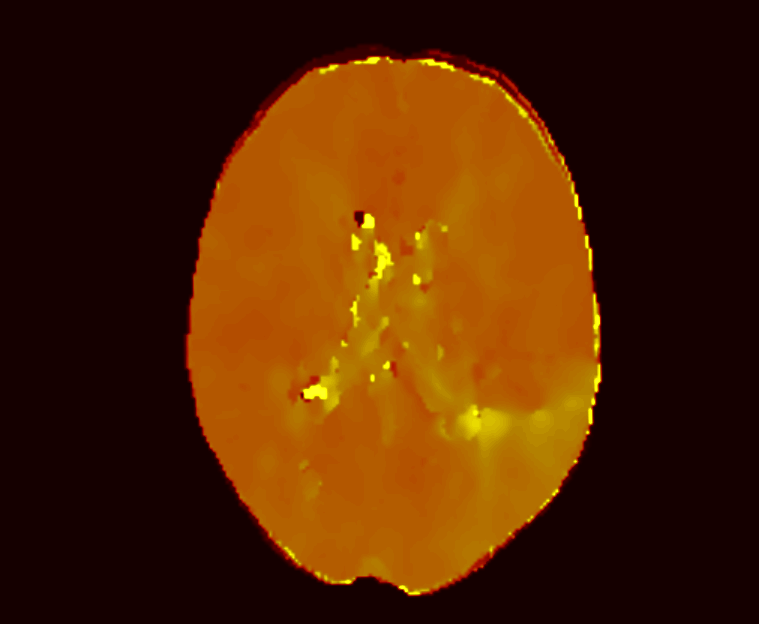
\includegraphics[width=\textwidth,height=4cm,keepaspectratio]{figures/perfusion_tmax.png}
        \caption{Time to Maximum (Tmax) map}
        \label{fig:tmax}
    \end{subfigure}
    \hfill
    \begin{subfigure}[t]{0.3\textwidth}
        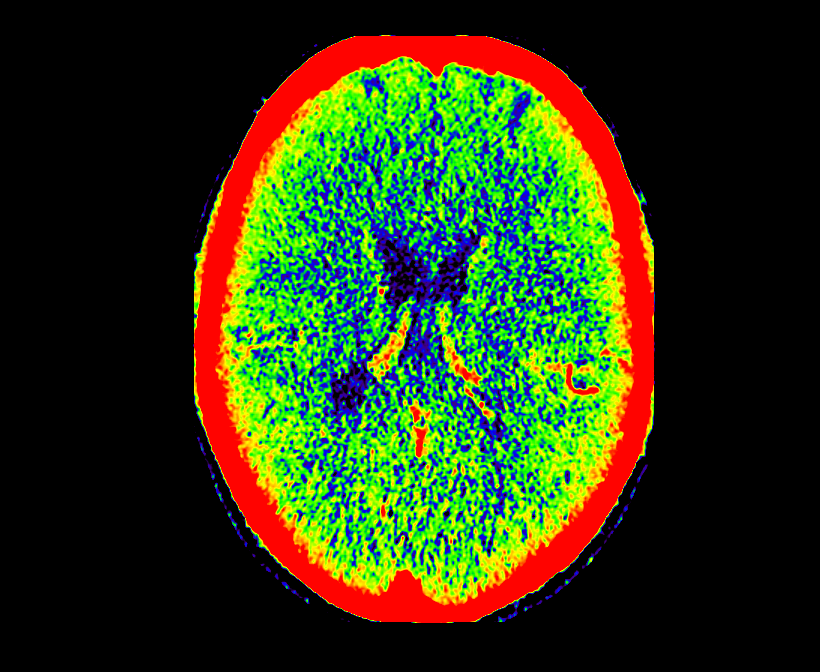
\includegraphics[width=\textwidth,height=4cm,keepaspectratio]{figures/perfusion_cta.png}
        \caption{CT Angiography (CTA) map}
        \label{fig:cta}
    \end{subfigure}
    \hfill
    \begin{subfigure}[t]{0.3\textwidth}
        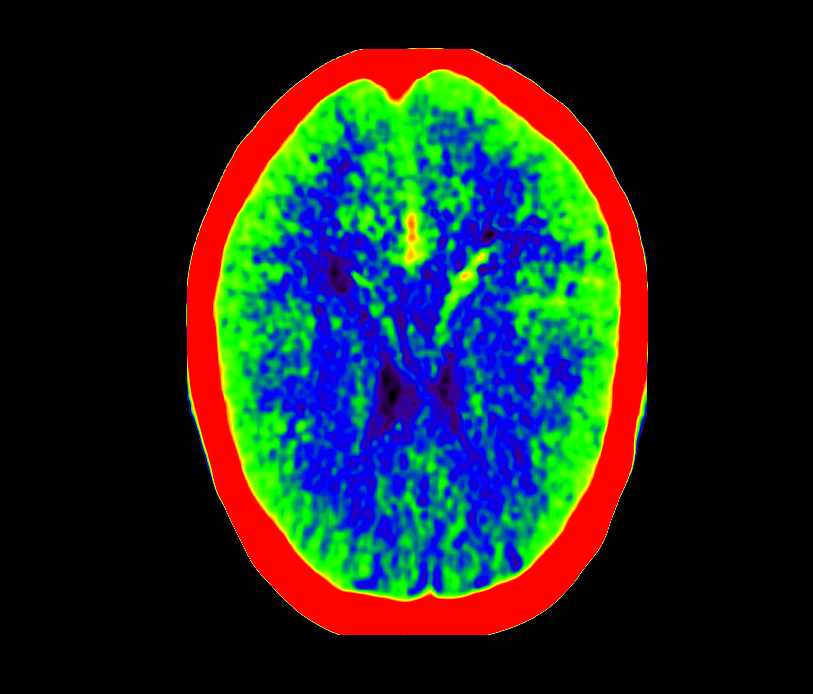
\includegraphics[width=\textwidth,height=4cm,keepaspectratio]{figures/perfusion_ctp.png}
        \caption{CT Perfusion (CTP) map}
        \label{fig:ctp}
    \end{subfigure}
    \caption{Different perfusion maps used in ischemic stroke analysis}
    \label{fig:perfusion_maps}
\end{figure}

\subsection{Technical Considerations}

Perfusion CT measures blood flow in the brain over time (every 1-2 seconds over 45-60 seconds) using a contrast agent. The derived perfusion maps help differentiate between irreversibly damaged (core) and salvageable (penumbra) tissue.

Different software packages use different deconvolution algorithms and thresholds, which can lead to varying estimations of core and penumbra volumes. This variability presents a challenge for standardization across clinical centers and research studies.

\section{Lesion Masks and Ground Truth}

Lesion masks represent binary infarct masks in the dataset and are derived from MRI images. They show the actual final infarct areas and are co-registered to the Non-Contrast CT (NCCT). These masks serve as ground truth—the target that predictive models aim to accurately reproduce based on earlier CT data. 